\chapter{Problem}
\label{ch:problem}

We define shape completion as the surface reconstruction of a single object
from a known object category given a partial observation of its shape
-- usually from one view only.
As indicated in the introduction, we follow a learning-based approach.
In its simplest form, \ie the supervised case, the problem can be
stated as:

\begin{problem}%[Supervised Shape Completion]
  \label{problem:supervised}
  Given (partial) observations $\mathcal{X} = \{x_1,\ldots,x_N\} \subseteq \mathbb{R}^R$ and
  shapes $\mathcal{Y}^* = \{y^*_1, \ldots, y^*_N\} \subseteq \mathbb{R}^R$ of a specific
  object category such that
  $y^*_n$ represents the ground truth shape of $x_n$, the task is to learn a 
  mapping $x_n \mapsto y^*_n$ that is able to generalize to previously unseen
  observations.
\end{problem}

Here, we assume the observations $x_n$ and shapes $y^*_n$ to be vectors in
some high-dimensional space $\mathbb{R}^R$ for brevity of notation. In practice,
we will resort to occupancy grids or signed distance functions in three spatial
dimensions, \eg $x_n, y^*_n \in \mathbb{R}^{H \times W \times D} \simeq \mathbb{R}^R$.
The observations $x_n$ correspond to observed points -- either
occupied or non-occupied -- and unobserved points. In order to make explicit
that these are merely partial observations, we use $x_n \in \{0,1,\uk\}^R$
where $\uk$ corresponds to unobserved points.

Obtaining the ground truth shapes $\mathcal{Y}^*$ for real-world
observations $\mathcal{X}$ is labor-intensive
(\cf \cite{GuptaMalik:2015,MenzeGeiger:2015}).
Thus, the unsupervised version of Problem \ref{problem:supervised} can be formulated
as follows:

\begin{problem}%[Unsupervised Shape Completion]
  \label{problem:unsupervised}
  Given (partial) observations $\mathcal{X} = \{x_1,\ldots,x_N\} \subseteq \mathbb{R}^R$
  of a specific object category,
  the task is to learn a mapping $x_n \mapsto y(x_n) \in \mathbb{R}^R$ where
  $y(x_n)$ represents a shape that matches the unknown ground truth
  shape $y^*_n \in \mathbb{R}^R$ as close as possible.
\end{problem}

Problem \ref{problem:unsupervised} can also be interpreted as weakly-supervised
problem as we assume knowledge about the object category. However, this knowledge
is not used explicitly yet. Furthermore, both
Problem \ref{problem:supervised} and Problem \ref{problem:unsupervised} imply that
each observation $x_n$ corresponds to one individual object. This
means that we assume an object detector to be given in order to extract
the observations $x_n$ from full point clouds
as provided in real-world applications, \eg on KITTI
\cite{GeigerLenzUrtasun:2012,GeigerLenzStillerUrtasun:2013}.

\section{Proposed Approach}

Problem \ref{problem:unsupervised} is inherently ambiguous; in practice, infinitely
many shapes may match a given observation and even the ground truth
shape does not need to match the observation perfectly due to noise.
We propose a Bayesian approach in order to model this uncertainty appropriately.
As we assume knowledge of the object category, we collect a set
$\mathcal{Y} = \{y_1, \ldots,y_M\} \subseteq \mathbb{R}^R$ of representative shapes
corresponding to this object category.
In practice, this might correspond to a set of Computer-Aided Design (CAD) models,
\ie triangular meshes. Problem \ref{problem:unsupervised} is then re-stated below:

\begin{figure}
  \centering
  \begin{tikzpicture}
    \node[rectangle,draw=black,fill=white] at (-3, 0.7) {
      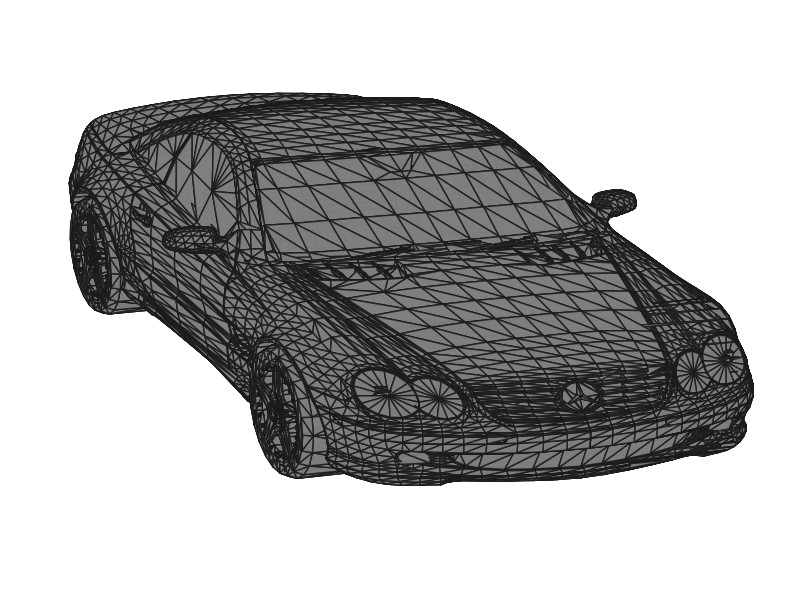
\includegraphics[height=1cm]{data/shapenet/simplification/119033fe083145e22f31600ac759c763}
    };
    \node[rectangle,draw=black,fill=white] at (-3, -0.7) {
      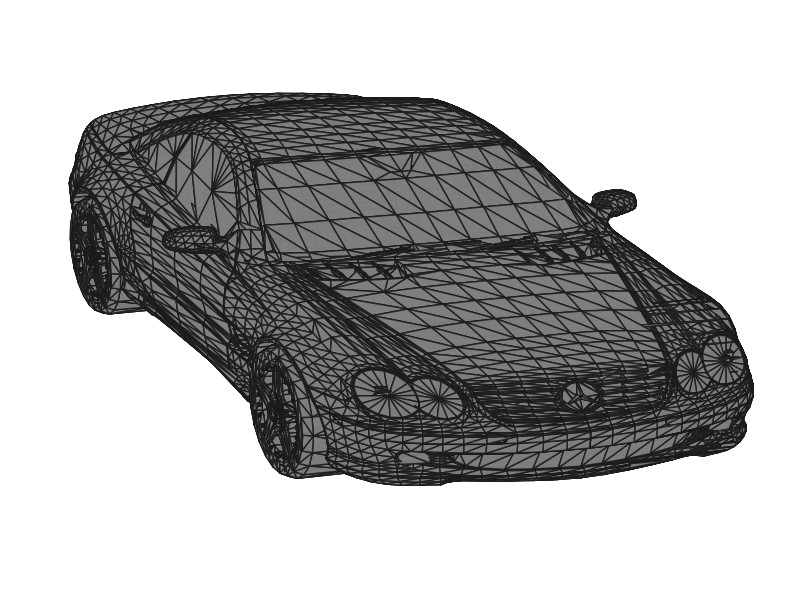
\includegraphics[height=1cm]{data/shapenet/simplification/119033fe083145e22f31600ac759c763}
    };
    \node[rectangle,draw=black,fill=white] at (-1.25, 0.7) {
      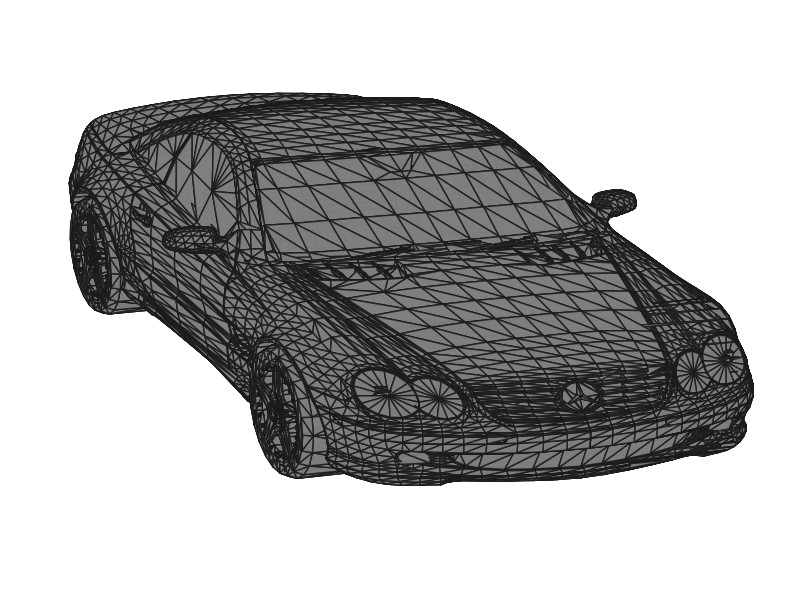
\includegraphics[height=1cm]{data/shapenet/simplification/119033fe083145e22f31600ac759c763}
    };
    \node[rectangle,draw=black,fill=white] at (-1.25, -0.7) {
      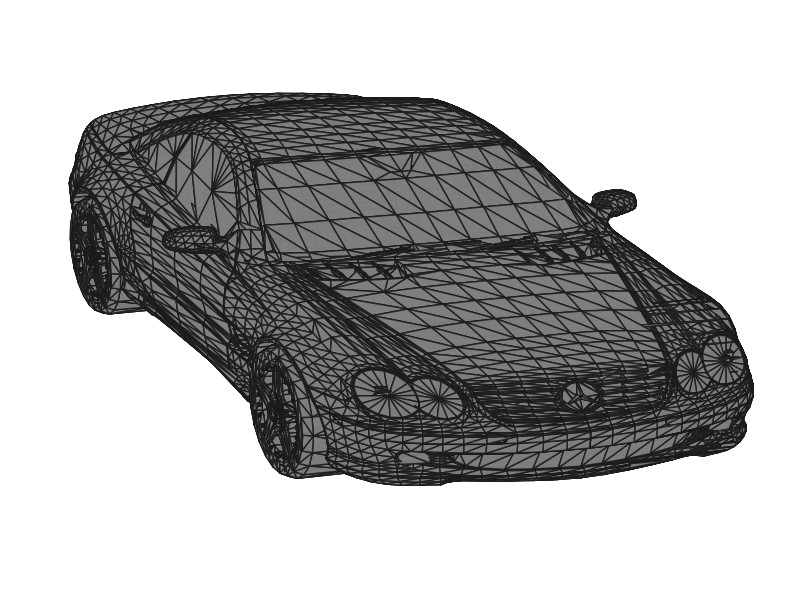
\includegraphics[height=1cm]{data/shapenet/simplification/119033fe083145e22f31600ac759c763}
    };
    \node at (-2.125, -1.75) {\small Shapes $y_m$};
    
    \node[rectangle,draw=black,fill=white] (input) at (1.4, 0) {
      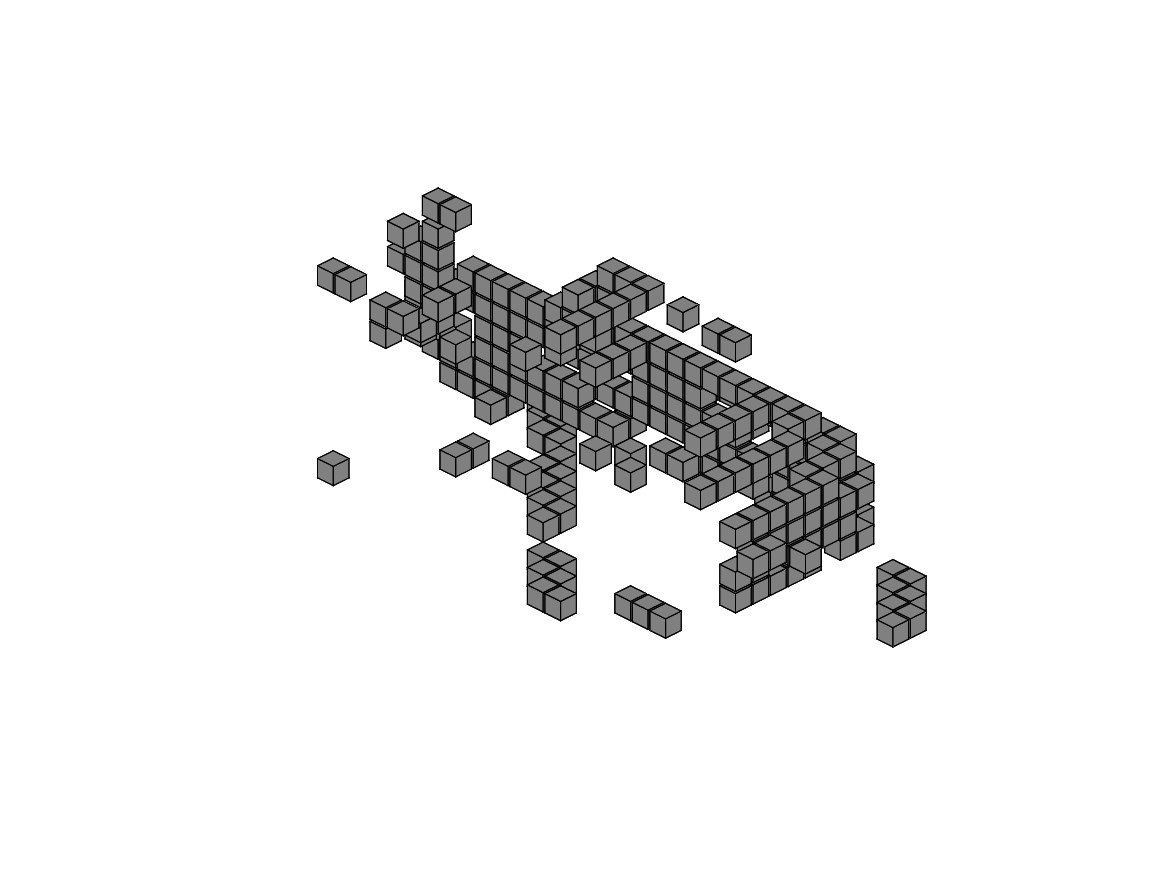
\includegraphics[height=2.4cm,trim={3cm 2cm 3cm 2cm},clip]{images/0_input_45}
    };
    \node at (1.4, -1.75) {\small Observation $x_n$};
    
    \node[rectangle,draw=black,fill=white] (output) at (8, 0) {
      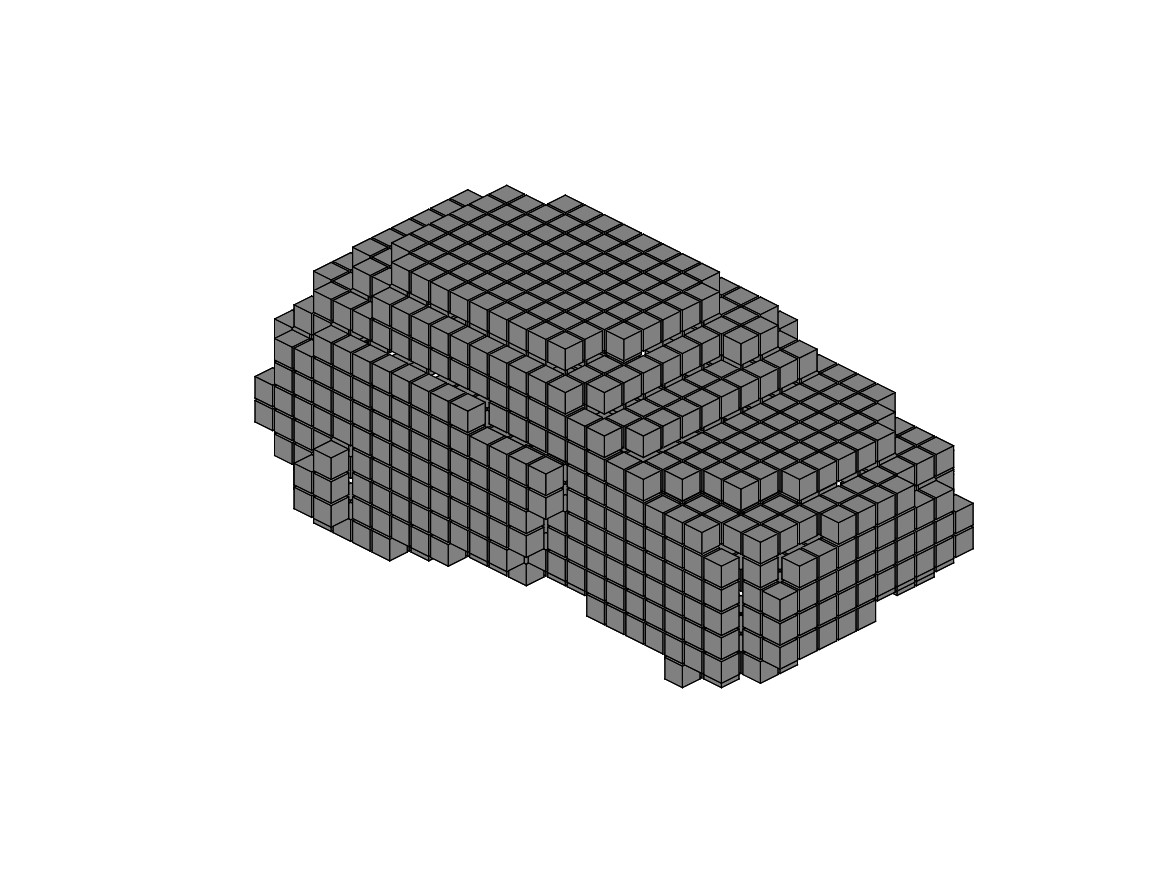
\includegraphics[height=2.4cm,trim={3cm 2cm 3cm 2cm},clip]{images/0_baseline_prediction_45}
    };
    \node at (8, -1.75) {\small Shape $y_n^*$};
    
    \node at (4.6, 0.65) {\small \begin{tabular}{c}Shape\\Completion\end{tabular}};
    \draw[->] (input) -- (output);
  \end{tikzpicture}
  \caption{An illustration of Problem \ref{problem}; the set of reference shapes
  $\mathcal{Y}$ is usually provided in the form of triangular meshes, \eg from
  ShapeNet \cite{ChangFunkhouserGuibasSavarese:2015}. After voxelization, these
  are used to learn a shape prior. The problem of shape completion is then
  illustrated by showing a voxelized observation $x_n$ and the
  corresponding ground truth, \ie completed, shape $y_n^*$.}
  \label{fig:problem}
\end{figure}

\begin{problem}%[Weakly-Supervised Shape Completion]
  \label{problem}
  Given (partial) observations
  $\mathcal{X} = \{x_1,\ldots,x_N\} \subseteq \mathbb{R}^R$
  and shapes $\mathcal{Y} = \{y_1, \ldots,y_M\} \subseteq \mathbb{R}^R$ of a specific object
  category, the task is to learn a mapping $x_n \mapsto y(x_n) \in \mathbb{R}^R$
  such that $y(x_n)$ matches the unknown ground truth
  shape $y^*_n \in \mathbb{R}^R$ as close as possible.
\end{problem}

We propose to use the set $\mathcal{Y}$ to learn a prior of possible shapes, \eg
using a variational auto-encoder. Shape completion can then be formulated as maximum
likelihood problem over a lower-dimensional latent space $\mathcal{Z} = \mathbb{R}^Q$,
$Q \ll R$. To this end, we interpret the individual voxels $y_i$, for $y \in \mathbb{R}^R$,
as random variables and $x_i$, for $x \in \mathbb{R}^R$, as the corresponding observations.
Then, $\mathcal{Y}$ is used to learn a prior model $p(y, z)$ which
decomposes into a generative model and a prior: $p(y, z) = p(y | z) p(z)$.
Using the set of observations $\mathcal{X}$, we then train an inference model
that directly learns the mapping
\begin{align}
  x \mapsto \tilde{z} = \argmax_{z} p(y = x | z) p(z).\label{eq:problem}
\end{align}
thereby implicitly solving Problem \ref{problem}. We interpret this approach
as amortized maximum likelihood following the idea of \cite{GershamGoodman:2014}.
In particular, we do not consider the maximum likelihood problem for each
observation $x$ independently. Instead, we understand the maximum likelihood
problem as loss between observations and shapes allowing to learn the
embedding $x \mapsto \tilde{z}$ in an unsupervised fashion. In the context
of variational auto-encoders, this boils down to training a new encoder to
represent the embedding of observations within the latent space.

Alternatively, we can consider the observations $x_i$ to be random variables, as well.
For the joint probability of the model, \ie $p(x, y, z)$, we can subsequently
derive the evidence lower bound. Using the simplifying assumption that $y$ and
$z$ are statistically independent given $x$, % \ie $q(y, z | x) = q(y | x) q(z | x)$,
we can use an extended variational auto-encoder to implicitly learn an approximate
model $q(z | x)$ which, again,
implicitly solves Problem \ref{problem}. Here, instead of directly
optimizing the maximum likelihood in Equation \eqref{eq:problem} (involving
$p(y = x | z)$), the observations are tied to the corresponding shapes through
a Kullback-Leibler divergence.
%In particular, the Kullback-Leibler
%divergence $\KL(q(y | x) | p(y | z))$ is minimized in order to learn
The learned model $q(z | x)$ can then be interpreted as a probabilistic embedding
of the observations in the latent shape space, in analogy to the
mapping $x \mapsto \tilde{z}$ learned when amortizing maximum likelihood.
Overall, both approaches require a shape prior defining a latent space
of shapes and subsequently learn to embed the partial observations within
this space.
